\documentclass{article}

\usepackage{amsmath}
\usepackage{amssymb}
\usepackage{graphicx}

\begin{document}


Ivan Lin\newline{}
Dr. Esther Arkin\newline{}
AMS301\newline{}
2/10/17

\begin{center}
  Homework 3b
\end{center}

\underline{Section 2.2 Problem 4}

Rules regarding Hamilton circuits:

Rule 1: If a vertex $x$ has degree 2, both of the edges touching $x$ must be part of any Hamilton circuit.

Rule 2: No proper subcircuit can be formed when building a Hamilton circuit.

Rule 3: Once a Hamilton circuit is required to use 2 edges at a vertex $x$, all other (unused) edges touching $x$ can be ignored (removed), as they cannot be used in a Hamilton circuit.

Theorem 1: If a graph G has a set S of $|S| = k$ vertices whose removal from G results in a graph $G_S$ which has more than k connected components, then G does not have a Hamilton circuit.

e. \newline{}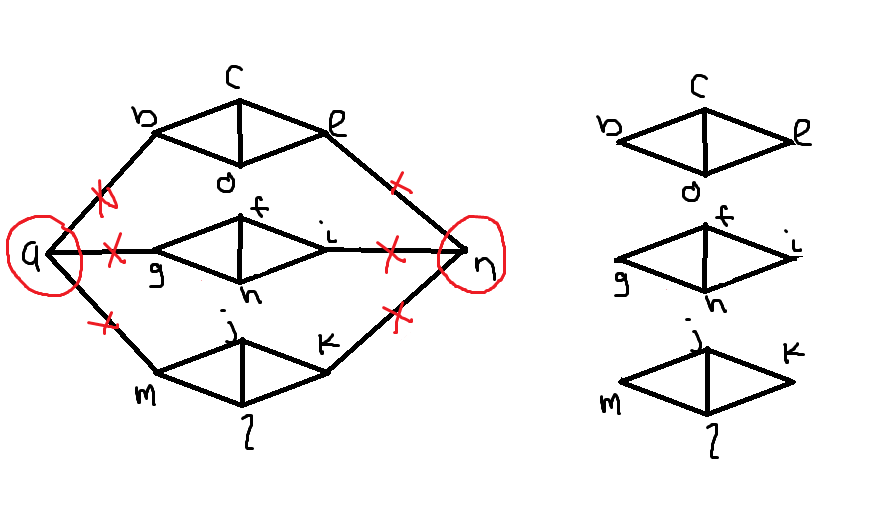
\includegraphics[height=150px]{hw2be.png}

By removing a the set of vertices $\{a,n\}$, three components are formed - $\{b,c,e,d\}$, $\{g,f,i,h\}$, $\{m,j,k,l\}$. By theorem 1, since the size of the set of removed vertices is 2 and its removal forms more than 2 components, the graph does not have a Hamilton circuit.

f. \newline{}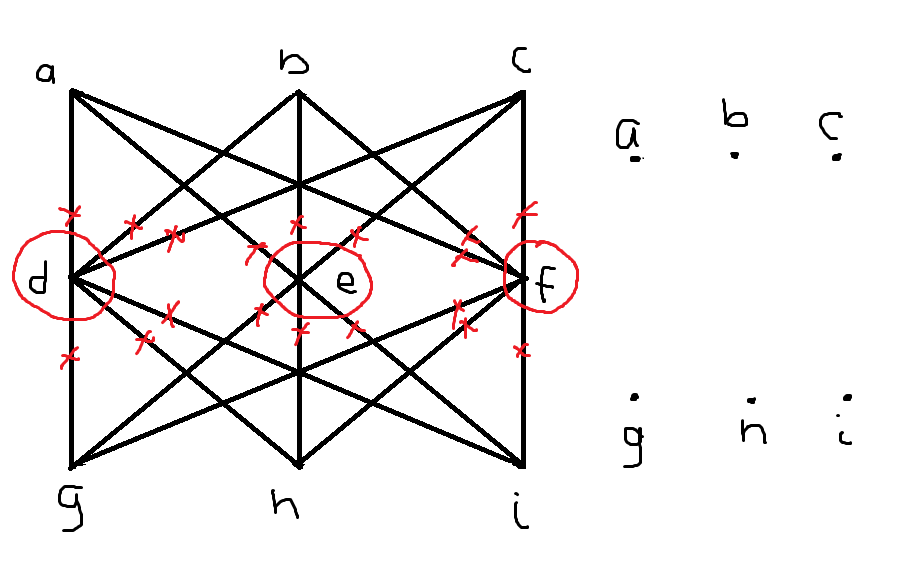
\includegraphics[height=150px]{hw2bf.png}

By removing a set of vertices $\{d,e,f\}$, six components are formed each consisting of a disconnected node $\{a\}$, $\{b\}$, $\{c\}$, $\{g\}$, $\{h\}$, $\{i\}$. By theorem 1, since the size of the set of removed vertices is 3 and its removal forms more than 3 components, the graph does not have a Hamilton circuit.

g. \newline{}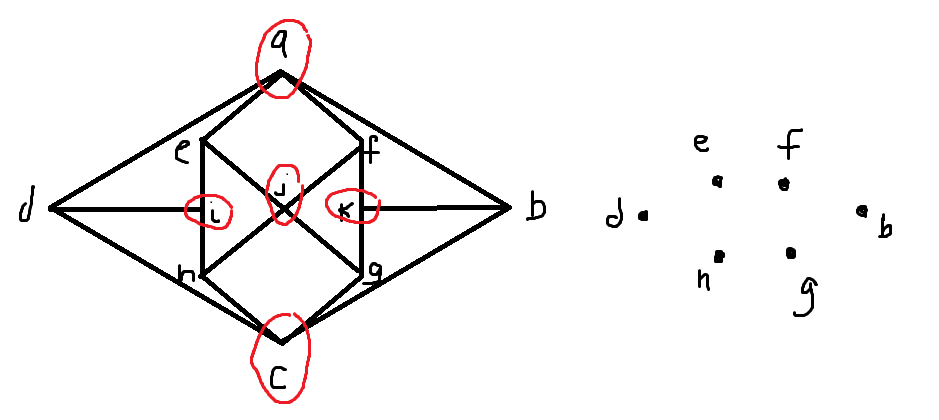
\includegraphics[height=150px]{hw2bg.png}

Bt removing a set of vertices $\{a,j,c,i,k\}$, six components are formed each consisting of a disconnected node $\{d\}$, $\{e\}$, $\{h\}$, $\{f\}$, $\{g\}$, $\{k\}$. By theorem 1, since the size of the set of removed vertices is 5 and its removal forms more than 5 components, the graph does not have a Hamilton circuit.

\end{document}
